\chapter{Algoritmi euristici}
In questo capitolo verranno trattati algoritmi euristici che non fanno uso di CPLEX. La necessità di non utilizzare CPLEX si ha per istanze con un numero elevato di nodi (10000-20000 nodi).\\
Per queste istanze la risoluzione del tableau attraverso CPLEX diventerebbe molto un'operazione molto onerosa per via dell'alto numero di variabili che verrano create e su cui verrà svolto il calcolo.\\
Attraverso gli algoritmi euristici, viene computata un'approssimazione della soluzione ottima e spesso però può essere sfruttata inizialmente dal risolutore CPLEX. Ad esempio questo può essere aggiunta prima della computazione, utilizzando la funzione \textit{CPXaddmipstarts()}, o ,se già definita, può essere modificata tramite \textit{CPXchgmipstarts()}.\\
Un algoritmo euristico, affinchè funzioni al meglio, deve essere composto da due fasi che si alternino:
\begin{itemize}
\item{\textbf{Intensificazione o raffinamento}\\
In questa fase la soluzione corrente viene migliorata fino al raggiungimento di un ottimo (locale o globale) nello spazio delle soluzioni.
}
\item{\textbf{Diversificazione}\\
Fase in cui la soluzioni viene perturbata con una politica predefinita affinchè si allontani da un ottimo locale nello spazio delle soluzioni.
}
\end{itemize}


\section{Euristici di costruzione}
Questa prima tipologia di algoritmi euristici è necessaria per la computazione di una prima soluzione ammissibile del problema.
\subsection{Nearest Neighborhood}
Questo algoritmo è basato su un approccio di tipo greedy.
L'algoritmo sceglie un nodo generico tra quelli che compongono il grafo. In seguito, iterativamente seleziona degli archi del grafo secondo il criterio enunciato nella seguente parte.\\
All'iterazione i-esima, vengono analizzati i costi degli archi che hanno un estremo pari al nodo selezionato all'iterazione i-1.\\
Viene selezionato l'arco che tra questi ha costo minore e il nuovo nodo raggiunto viene impostato come punto di partenza per analizzare i costi degli archi all'iterazione successiva (vedi Figura \ref{nearest_neighborhood}). All'ultima iterazione viene scelto l'arco che collega l'ultimo nodo visitato al nodo scelto inizialmente.\\
Il problema di questo algoritmo è che in ogni iterazione viene selezionato esclusivamente il vertice più vicino a quello scelto precedentemente, senza però prevedere la futura evoluzione del ciclo, creato dall'algoritmo.\\
Come in Figura \ref{nearest_neighborhood}, la scelta dell'arco di costo minimo non implica che in seguito venga generata la soluzione ottima. Scegliendo un nodo iniziale differente, viene generato un tour differente.\\
Definito \textbf{n} come il numero di nodi presenti nel grafo, si avranno quindi n soluzioni differenti, ottenute ciascuna attraverso n iterazioni dell'algoritmo. In seguito tra queste possibli soluzioni, verrà selezionata quella di costo minore.\\
\begin{figure}[h] 
\begin{center} 
  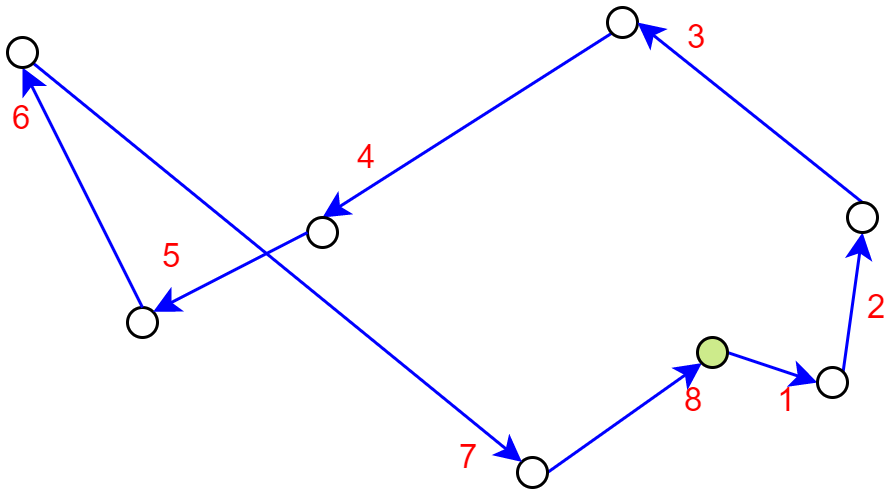
\includegraphics[scale=0.4]{Images/nearest_neighborhood}\\ 
  \caption{\footnotesize{Esempio di esecuzione di Nearest Neighborhood.}}
  \label{nearest_neighborhood} 
\end{center} 
\end{figure}
Per migliorare l'algoritmo viene aggiunta una scelta aleatoria, utilizzando il metodo Greedy Adaptive Search Procedure (GASP). Ad ogni iterazione, invece di selezionare l'arco di costo minimo, vengono messi in evidenza i tre archi con costo minore e ne viene selezionato casualmente uno tra questi.\\
Un'implementazione alternativa invece fa uso sia del metodo standard che del metodo GASP. In questo caso la scelta casuale non viene fatta su ogni iterazione ma con una certa periodicità fissata inizialmente.

\subsection{Heuristic Insertion}
L'algoritmo seguente usa un approcco simile al precedente ma prevede la selezione di un ciclo iniziale a cui apportare modifiche, per ottenere una soluzione iniziale ammissibile del problema. Per definire il ciclo di partenza vengono utilizzati diversi metodi. Di seguito sono riportati i due più utilizzati:
\begin{itemize}
\item{\textbf{Selezione di due nodi}\\
Vengono scelti i due nodi più lontani tra loro nel grafo o due nodi casuali e  sono selezionati i due archi orientati che li collegano.
}
\item{\textbf{Inizializzazione geometrica}\\
Nel caso in cui i nodi siano punti 2D, può essere calcolata la convex-hull e utilizzarla come ciclo iniziale. 
}
\end{itemize}
In seguito a tale operazione, questa soluzione viene modificata iterativamente. Per ogni coppia di nodo non appartenente al ciclo \textbf{C}, restituito dall'iterazione precedente, viene calcolato l'extramileage $\Delta_h$ come segue:
$$\Delta_h = \underset{(a,b)\in C}{min} c_{ah}+c_{hb}-c_{ay}$$
con $c_ij$ costo dell'arco che collega i a j (vedi Figura \ref{partial_cycle}).\\
Alla fine di ciascuna iterazione viene aggiunto nel grafo il nodo \textbf{k} che minimizza l'\textbf{extramileage} (vedi Figura \ref{insertion}):\\
$$k = arg\underset{h}{min}\Delta_{h}$$
Un modo per aggiungere aleatorietà a questo algoritmo può essere quello di sfruttare l'approccio GASP nella selezione del minimo extramileage. Il nodo da aggiungere in un'iterazione al grafo, viene selezionato in modo casuale tra i tre con $\Delta$ minore.
\begin{figure}[h] 
\begin{center} 
  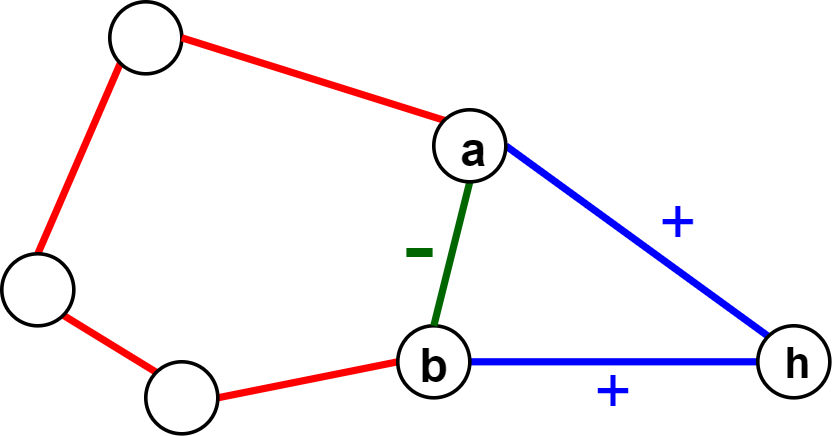
\includegraphics[scale=0.2]{Images/partial_cycle}\\ 
  \caption{\footnotesize{Parte del calcolo dell'extramileage del nodo \textbf{h}.}}
  \label{partial_cycle}
\end{center}
\end{figure}
\begin{figure}[h] 
\begin{center} 
  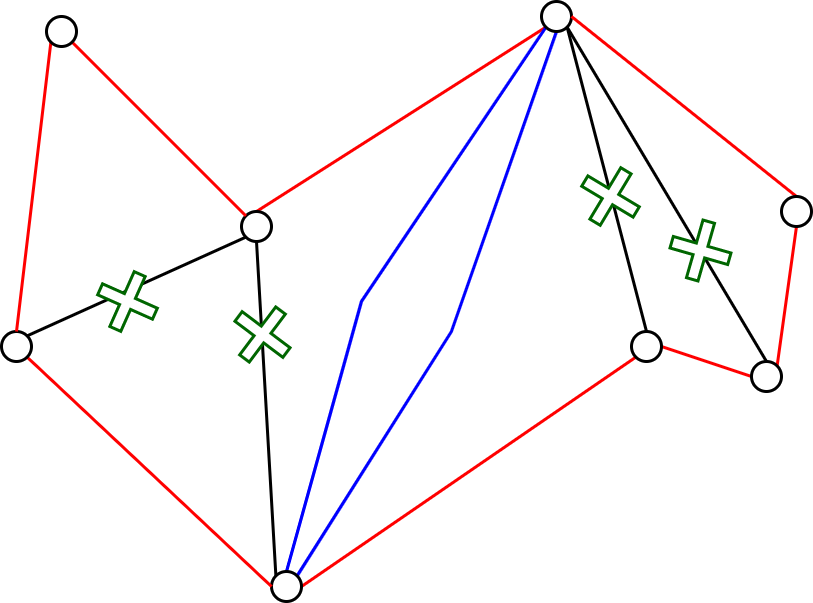
\includegraphics[scale=0.4]{Images/insertion}\\ 
  \caption{\footnotesize{Esempio dell'applicatione di Heuristic insertion.}}
  \label{insertion}
\end{center}
\end{figure}
\section{Algoritmi di raffinamento}
Una volta ottenuto una prima soluzione è necessario migliorarla per avvicinarsi il più possibile all'ottimo. Gli algoritmi utilizzati con questo scopo sono detti \textit{di raffinamento}. Nel capitolo precedente sono già stati descritti due procedimenti di questo tipo, l'Hard Fixing e il Soft Fixing (vedi sottosezioni \ref{hard fixing} e \ref{soft fixing}). In questa sezione verranno invece analizzati algoritmi di raffinamento che non utilizzino funzioni messe a disposizione da CPLEX.
\subsection{Algoritmo di 2 ottimalità}
Nelle soluzioni restituite dagli algoritmi euristici di costruzione sono spesso presenti incroci tra rami che colleghino coppie di nodi appartenenti al circuito. La loro presenza implica sempre la non ottimalità della soluzione, in quanto per le proprietà dei triangoli esisterà sempre una soluzione che eviti l'incrocio e che sia di costo minore (vedi figura \ref{cross}). 
\begin{figure}[h] 
\begin{center} 
  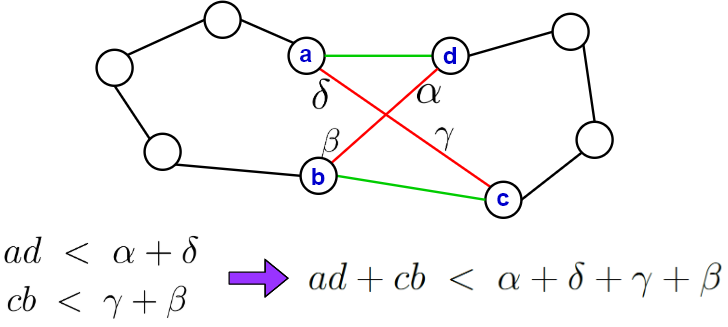
\includegraphics[scale=0.4]{Images/triangle_property}\\ 
  \caption{\footnotesize{Accenno alla dimostrazione della non ottimalità di una soluzione con incrocio.}}
  \label{cross}
\end{center}
\end{figure}
Il procedimento qui descritto si pone l'obiettivo di trovare questa soluzione. Poichè la soluzione che trova si differenzia dalla precedente sempre solo per due rami (quelli che nella prima formavano l'incrocio) viene detto algoritmo di 2 ottimalità.\\
Nell'implementazione del procedimento non è necessario cercare tutti gli incroci della soluzioni per eliminarli, ma è sufficiente analizzare tutte le coppie di rami presenti e verificare se, scambiandole con un'altra coppia ammissibile, si verifica un miglioramento.
\begin{figure}[h] 
\begin{center} 
  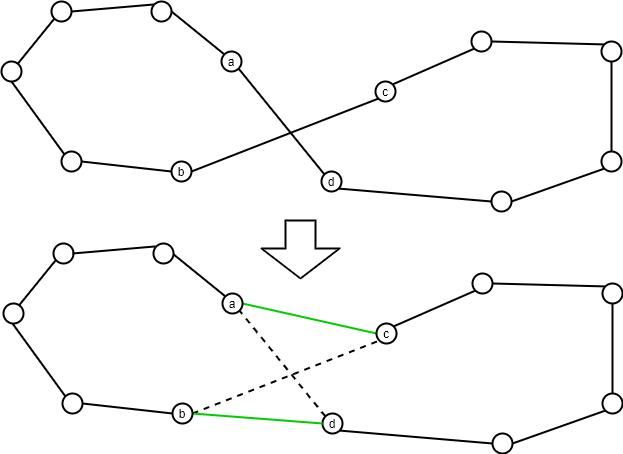
\includegraphics[scale=0.3]{Images/switch}\\ 
  \caption{\footnotesize{Esempio di eliminazione di un incrocio.}}
  \label{switch}
\end{center}
\end{figure}
Riferendosi alla figura \ref{switch}, questo viene così calcolato:\\
 $$\Delta = (c_{ac} + c_{bd}) - (c_{ad} + c_{bc})$$
 Solo nel caso in cui risulti $\Delta < 0$ la sostituzione viene memorizzata.\\
In questo modo ogni nuova soluzione appartiene all'intorno di 2 ottimalità, della soluzione precedente, nello spazio delle soluzioni. Aggiornando iterativamente la soluzione si raggiunge un ottimo locale, ovvero in cui non sono possibili miglioramenti nel costo della soluzione, modificando una sola coppia di rami. Questo spostamento è rappresentato in Figura \ref{two_optimality}. 
\begin{figure}[h] 
\begin{center} 
  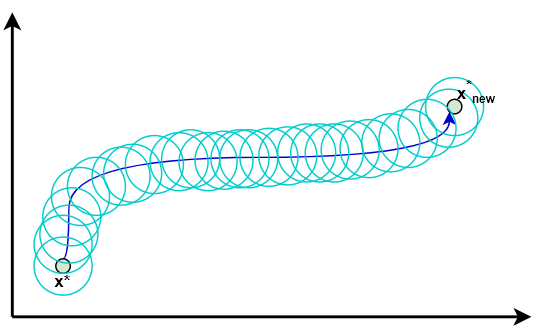
\includegraphics[scale=0.4]{Images/two_optimality}\\ 
  \caption{\footnotesize{Aggiornamento della soluzione in intorni di 2 ottimalità.}}
  \label{two_optimality}
\end{center}
\end{figure}
Un analogo procedimento viene utilizzato anche nell'algoritmo Soft Fixing, in cui però la dimensione dell'intorno in cui cercare la nuova soluzione può variare (vedi Figura \ref{local_exe}).\\
Poichè per il calcolo del $\Delta$ avviene in tempo costante e deve essere fatto per ogni coppia di rami, il tempo complessivo per la computazione è $O(n^2)$, con $n$ nodi nell'istanza del problema.
\subsection{Algoritmo di 3 ottimalità}
L'algoritmo di 3 ottimalità è analogo a quello analizzato nella sezione precedente, ma considera intorni di 3 ottimalità, nello spazio delle soluzioni, per aggiornare il circuito corrente. In questo caso, quindi, due soluzioni si differenziano per 3 rami, che devono essere scelti con particolare attenzione essendo in maggior numero le possibilità di scelta (vedi Figura \ref{three_optimality}).
\begin{figure}[h] 
\begin{center} 
  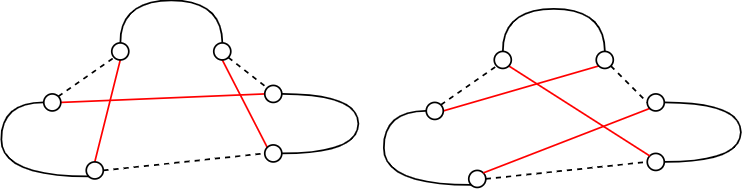
\includegraphics[scale=0.4]{Images/three_exchange}\\ 
  \caption{\footnotesize{Due possibile combinazioni di scelta dei nuovi rami da inserire nella soluzioni.}}
  \label{three_optimality}
\end{center}
\end{figure}
Rimanendo comunque in quantità costante, l'algoritmo impiega in tutto $O(n^3)$ (con $n$ numero di nodi) per trovare un ottimo locale, essendo $O(n^3)$ il numero di terne di rami esistenti. Su istante con un alto numero di nodi, questo tempo computazione può essere troppo elevato per il calcolo di una soluzione. 
\section{Meta-euristici}
Gli algoritmi di raffinamento appena visti si occupano di migliorare il più possibile una soluzione già calcolata attraverso meccanismi di local serch. In questo modo, dopo un determinato numero di iterazioni, viene raggiunto un ottimo locale. Le metodologie che vengono descritte in questa sezione cercano di aggiornare questa soluzione allontanandola dall'ottimo locale e convogliandola in un ottimo globale, se possibile. Possono quindi essere descritti come algoritmi euristici per progettare altri euristici, per definizione non sono quindi in grado di garantire il raggiungimento dell'ottimo globale.\\
Questi procedimenti sono più generali di quelli descritti fin'ora, applicabili anche ad istanze di problemi diversi e non solo del commesso viaggiatore. 
\subsection{Multi-starting}
Un primo e intuitivo approccio per allontanarsi da un ottimo locale è quello descritto  dalla politica multi-starting: applicare l'algoritmo di raffinamento scelto a diverse soluzioni iniziali. In questo modo si raggiungono ottimi locali diversi (come mostrato in Figura \ref{multi_starting})e viene restituita la soluzione corrispondente al costo minore. 
\begin{figure}[h] 
\begin{center} 
  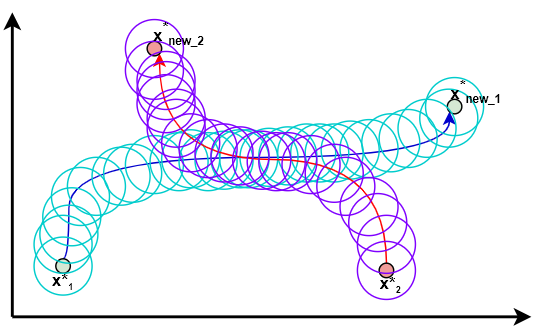
\includegraphics[scale=0.5]{Images/multistarting}\\ 
  \caption{\footnotesize{Due possibile esecuzioni di un algoritmo di raffinamento con partenze da due soluzioni diverse.}}
  \label{multi_starting}
\end{center}
\end{figure}
Un aspetto negativo di questo approccio, però, è il fatto che ogni volta che viene selezionata una soluzione di partenza diversa si perdono le informazioni ottenute dalla computazione precedente che ha già raggiunto un ottimo locale.
\subsection{Variable Neighborhood Search \cite{VNS}}
Una volta ottenuta una soluzione corrispondente ad un ottimo locale nella funzione di costo si può cercare di migliorarla analizzando i suoi intorni di ottimalità di raggio crescente. Questo però non garantisce un effettivo cambiamento della soluzione. Il Variable Neighborhood Search (VNS) è un algoritmo che sfrutta questa ricerca. Nel caso non si verifichi un aggiornamento della soluzione prevede che vengano scelti un certi numero di rami randomici da sostituire con altri non appartenenti alla soluzione, in maniera casuale. In questo modo si impone un aggiornamento con una crescita del costo, nella speranza che nel nuovo intorno selezionato sia possibile trovare una soluzione che si allontani dall'iniziale ottimo locale (Figura \ref{VNS}).\\
 \begin{figure}[H] 
\begin{center} 
  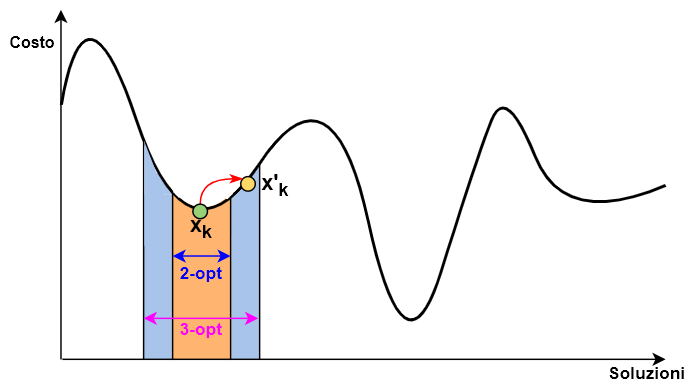
\includegraphics[scale=0.5]{Images/VNS_bianco}\\ 
  \caption{\footnotesize{Aggiornamento di una soluzione in un minimo locale.}}
  \label{VNS}
\end{center}
\end{figure}
L'algoritmo termina allo scadere del tempo a disposizione o dopo un determinato numero di iterazione, restituendo la miglior soluzione trovata fino a quel momento.\\
Utilizzando questo approccio gran parte della soluzione di partenza viene conservata evitando di perdere le informazioni elaborate precedentemente all'utilizzo di VNS.
\subsection{Tabu search \cite{Tabu}}%inserire nostra implementazione delle mosse vietate
L'approccio Tabu search fu ideato da Fred W. Glover. Data una soluzione in un ottimo locale dello spazio delle soluzioni, l'idea di Glover permette di aggiornarla anche con una di costo più elevato (generalmente si cerca di minimizzare questo peggioramento). Per evitare che all'iterazione successiva si ritorni nella soluzione di partenza, viene creata una lista di "mosse vietate" , detta Tabu list, che impedisca di raggiungere nuovamente l'ottimo locale. In questo modo la soluzione aumenta di costo per un certo numero di iterazioni, finchè non ricomincia a diminuire per raggiungere un nuovo minimo locale o globale. Nel caso in cui si incontri una soluzione che migliori l'incumbent senza rispettare tutti i vincoli presenti nella Tabu list, l'algoritmo aggiorna ugualmente la soluzione corrente. Questo meccanismo viene detto \textit{Aspiration criterion}.\\ 
Aumentando costantemente di dimensione la lista Tabu si rischia, ad un certo punto, che non sia più possibile aggiornare la soluzione. Per evitare ciò generalmente viene scelta una capienza massima (detta \textit{tenure}) della lista, una volta raggiunta la lista viene aggiornata rispettando la politica FIFO (first in first out). Per far si che l'algoritmo oscilli tra la fase di diversificazione e quella di intensificazione, la tenure viene fatta variare durante le diverse iterazioni tra due valori (massimo e minimo) (vedi Figura \ref{tenure}). Nelle iterazioni in cui è massima si verifica la diversificazione, in quelle in cui è minima l'intensificazione. Se viene applicata questa scelta implementativa l'algoritmo è chiamato \textit{Reactive Tabu Search}.
 \begin{figure}[H] 
\begin{center} 
  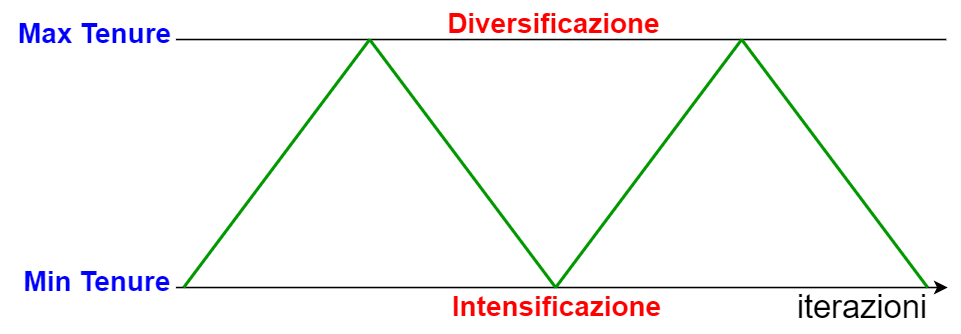
\includegraphics[scale=0.35]{Images/tenure}\\ 
  \caption{\footnotesize{Variazione della tenure.}}
  \label{tenure}
\end{center}
\end{figure}
Come per l'algoritmo precedente, il criterio di terminazione è dato dallo scadere del tempo a disposizione o dal raggiungimento del numero massimo di iterazioni scelto, restituendo la miglior soluzione trovata fino a quel momento.\\
\subsection{Simulated annealing}%citazione? trovare articolo?
L'algoritmo simulated annealign, come dice il nome, è ispirato dal processo di temperamento dei metalli, in cui il materiale viene raffreddato molto lentamente e in maniera controllata, affinchè raggiunga la configurazione di minima energia. Analogamente, in questo algoritmo viene scelta una funzione (generalmente esponenziale) che descriva la variazione della "temperatura" $T$. Ad ogni iterazione la soluzione corrente può essere aggiornata con una qualsiasi altra interna all'intorno di 2 ottimalità, di costo minore o maggiore, con una probabilità funzione della variazioni di costo e della temperatura attuale, $f(\Delta costo, T)$. Questo implica che non sia necessario scandire tutto l'intorno, ma che sia sufficiente scegliere in maniera randomica 2 rami da sostituire nella soluzione (Figura \ref{simulated_annealing}).
 \begin{figure}[H] 
\begin{center} 
  \includegraphics[scale=0.6]{Images/simulated_anneling_bianco}\\ 
  \caption{\footnotesize{Esempio di esecuzione dell'algoritmo Simulated Annealing.}}
  \label{simulated_annealing}
\end{center}
\end{figure}
 Con il procedere delle iterazioni, l'aggiornamento ad un costo peggiore avviene sempre meno frequentemente, fino ad ottenere solo aggiornamenti con soluzioni più vantaggiose. Esiste un teorema secondo il quale se la temperatura varia in maniera estremamente lenta ed è consentito effettuare un numero di iterazioni estremamente elevato, questo algoritmo garantisce di trovare l'ottimo globale. Concretamente queste ipotesi sono molto difficili da realizzare, ma è statisticamente comunque possibile dichiarare che l'approccio del simulated annealing restituisce una buona soluzione.
\section{Funzione di costo a scalini}
La funzione obiettivo di un problema può avere, in particolari circostanze, un grafico a scalini, in cui cioè esistano diverse soluzioni dell'istanza con lo stesso costo. In questo caso è consigliabile applicare una politica che utilizzi delle penalità per perturbare la funzione affinché non siano più presenti le zone costanti, che potrebbero causare problemi nell'aggiornamento della soluzione da restituire. Generalmente questa situazione non si verifica con istanze del problema del commesso viaggiatore in cui i costi dipendono dalla distanza euclidea. Nel caso fosse necessario, però, è possibile ammettere che l'algoritmo utilizzato per la risoluzione del problema, restituisca anche soluzioni con più componenti connesse. In questo modo sarebbe possibile scegliere una penalità dipendente dal numero di vincoli violati (ovvero dal numero di subtour presenti) che influenzi il costo della soluzione nel seguente modo:
$$costo\_totale = costo\_archi + M (num\_subtour -1)$$
con M variabile molto grande.